% ============================================================================
%  ADVANCED COMPUTER ARCHITECTURE ACADEMIC STUDENT NOTES
%  UNIT 2: Principles of Scalable Performance & Processor Technology
% ============================================================================

\documentclass[11pt,a4paper]{article}

% ── Fonts ───────────────────────────────────────────────────────────────────
\usepackage[T1]{fontenc}
\usepackage{noto}

% ── Page Layout ─────────────────────────────────────────────────────────────
\usepackage[
  a4paper,
  left=1in,
  right=1in,
  top=1.15in,
  bottom=1.15in,
  headheight=22pt
]{geometry}

% ── Colors ──────────────────────────────────────────────────────────────────
\usepackage[dvipsnames,svgnames,table]{xcolor}

\definecolor{TheoremBlue}{RGB}{0,82,155}
\definecolor{DefinitionGreen}{RGB}{0,112,74}
\definecolor{ExampleOrange}{RGB}{184,84,0}
\definecolor{RemarkPurple}{RGB}{108,52,131}
\definecolor{ProofBorder}{RGB}{120,120,160}
\definecolor{NoteRed}{RGB}{179,0,0}
\definecolor{ChapterBlue}{RGB}{20,60,120}

% ── Math Packages ───────────────────────────────────────────────────────────
\usepackage{amsmath,amssymb,amsthm,mathtools}
\usepackage{mathrsfs}
\usepackage{bbm}

% ── Theorem Environments (tcolorbox) ────────────────────────────────────────
\usepackage[most]{tcolorbox}
\tcbuselibrary{theorems, skins, breakable}

\newtcbtheorem[number within=section]{theorem}{Theorem}{%
  enhanced,
  colback=TheoremBlue!4,
  colframe=TheoremBlue!80!black,
  coltitle=white,
  fonttitle=\bfseries,
  sharp corners,
  boxrule=0.8pt,
  top=6pt, bottom=6pt, left=8pt, right=8pt,
  separator sign none,
  description delimiters parenthesis,
  breakable
}{thm}

\newtcbtheorem[number within=section]{definition}{Definition}{%
  enhanced,
  colback=DefinitionGreen!4,
  colframe=DefinitionGreen!70!black,
  coltitle=white,
  fonttitle=\bfseries,
  rounded corners,
  boxrule=0.8pt,
  top=6pt, bottom=6pt, left=8pt, right=8pt,
  separator sign none,
  description delimiters parenthesis,
  breakable
}{def}

\newtcbtheorem[number within=section]{example}{Example}{%
  enhanced,
  colback=ExampleOrange!4,
  colframe=ExampleOrange!60!black,
  fonttitle=\bfseries,
  rounded corners,
  boxrule=0.6pt,
  borderline west={3pt}{0pt}{ExampleOrange!80},
  top=5pt, bottom=5pt, left=10pt, right=8pt,
  separator sign none,
  breakable
}{ex}

\newtcolorbox{remark}[1][]{%
  enhanced,
  colback=RemarkPurple!3,
  colframe=RemarkPurple!3,
  borderline west={2.5pt}{0pt}{RemarkPurple!70},
  sharp corners,
  boxrule=0pt,
  top=5pt, bottom=5pt, left=8pt, right=8pt,
  fontupper=\small,
  before upper={\textbf{\color{RemarkPurple}Remark.}\quad},
  breakable,
  #1
}

\newtcolorbox{notebox}[1][]{%
  enhanced,
  colback=NoteRed!3,
  colframe=NoteRed!3,
  borderline west={2.5pt}{0pt}{NoteRed!70},
  sharp corners,
  boxrule=0pt,
  top=5pt, bottom=5pt, left=8pt, right=8pt,
  before upper={\textbf{\color{NoteRed}Note.}\quad},
  breakable,
  #1
}

% ── TikZ Diagrams ───────────────────────────────────────────────────────────
\usepackage{tikz}
\usetikzlibrary{positioning, arrows.meta, shapes.geometric, calc, fit, backgrounds}

\tikzset{
  box/.style={draw, rectangle, rounded corners, fill=blue!10, minimum width=2.2cm, minimum height=1cm, align=center, font=\small},
  mem/.style={draw, rectangle, fill=green!10, minimum width=4cm, minimum height=1cm, align=center, font=\small},
  net/.style={draw, double, fill=orange!10, minimum width=6cm, minimum height=0.8cm, align=center, font=\small\bfseries},
  node/.style={circle, draw=blue!80, fill=blue!15, minimum size=8mm, font=\small\bfseries}
}

% ── Lists ───────────────────────────────────────────────────────────────────
\usepackage[shortlabels]{enumitem}
\setlist[enumerate]{topsep=4pt, itemsep=2pt, parsep=2pt}
\setlist[itemize]{topsep=4pt, itemsep=2pt, parsep=2pt}
\setlist[enumerate,1]{label=\arabic*.}

% ── Tables ──────────────────────────────────────────────────────────────────
\usepackage{booktabs}
\usepackage{array}
\usepackage{tabularx}

% ── Headers and Footers ────────────────────────────────────────────────────
\usepackage{fancyhdr}
\pagestyle{fancy}
\fancyhf{}
\fancyhead[L]{\color{gray}\small UNIT 2: Principles of Scalable Performance}
\fancyhead[R]{\color{gray}\small Advanced Computer Architecture}
\fancyfoot[C]{\thepage}
\renewcommand{\headrulewidth}{0.4pt}
\renewcommand{\footrulewidth}{0pt}

% ── Section Styling ─────────────────────────────────────────────────────────
\usepackage{titlesec}
\titleformat{\section}
  {\Large\bfseries\color{ChapterBlue}}
  {\thesection}{0.8em}{}

\titleformat{\subsection}
  {\large\bfseries\color{DefinitionGreen!80!black}}
  {\thesubsection}{0.8em}{}

% ── Hyperlinks & Cross-references ───────────────────────────────────────────
\usepackage[colorlinks=true, linkcolor=TheoremBlue, citecolor=TheoremBlue, urlcolor=TheoremBlue]{hyperref}
\usepackage[nameinlink,capitalize]{cleveref}

% ============================================================================
%  DOCUMENT BEGINS
% ============================================================================
\begin{document}

\begin{titlepage}
\centering
\vspace*{1.5cm}

{\color{ChapterBlue}\rule{\textwidth}{1.5pt}}
\vspace{0.6cm}
{\fontsize{26}{32}\selectfont\bfseries\color{ChapterBlue} Advanced Computer Architecture}
\vspace{0.4cm}
{\Large\color{gray} Academic Student Notes}
\vspace{0.4cm}
{\color{ChapterBlue}\rule{\textwidth}{1.5pt}}

\vspace{1cm}
{\large\textbf{UNIT - II: Principles of Scalable Performance \& Hardware Technologies}}

\vspace{1.5cm}

\begin{center}
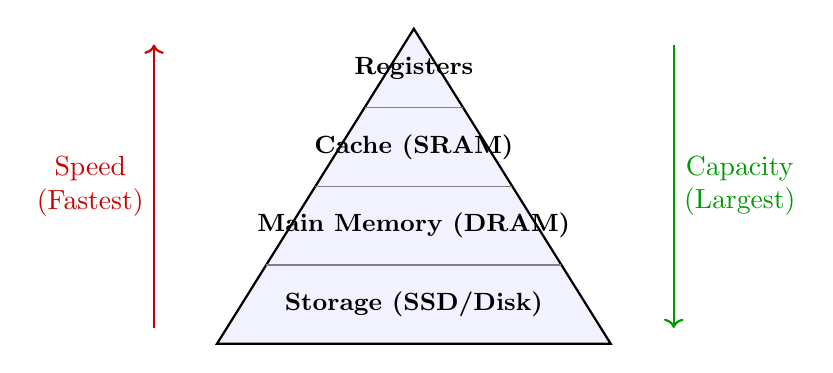
\begin{tikzpicture}[scale=1.0]
  % Memory Hierarchy Pyramid
  \draw[thick, fill=blue!5] (0,0) -- (5,0) -- (2.5,4) -- cycle;
  
  % Horizontal slices
  \draw[gray] (0.625, 1.0) -- (4.375, 1.0);
  \draw[gray] (1.25, 2.0) -- (3.75, 2.0);
  \draw[gray] (1.875, 3.0) -- (3.125, 3.0);
  
  % Labels
  \node[font=\small\bfseries] at (2.5, 3.5) {Registers};
  \node[font=\small\bfseries] at (2.5, 2.5) {Cache (SRAM)};
  \node[font=\small\bfseries] at (2.5, 1.5) {Main Memory (DRAM)};
  \node[font=\small\bfseries] at (2.5, 0.5) {Storage (SSD/Disk)};
  
  % Side Arrows
  \draw[thick, ->, red!80!black] (-0.8, 0.2) -- (-0.8, 3.8) node[midway, left, align=center] {Speed \\ (Fastest)};
  \draw[thick, ->, green!60!black] (5.8, 3.8) -- (5.8, 0.2) node[midway, right, align=center] {Capacity \\ (Largest)};
\end{tikzpicture}
\end{center}

\vspace{1.5cm}
{\large\textit{Department of Computer Science and Engineering}} \\
\vspace{0.2cm}
{\large\textbf{Marri Laxman Reddy Institute of Technology and Management}} \\
\vspace{0.1cm}
{\small (UGC Autonomous, R25 Regulation)}

\vfill
{\normalsize Compiled: \today}
\end{titlepage}

\tableofcontents
\newpage

% ============================================================================
\section{Performance Metrics and Measures}
% ============================================================================

To evaluate how well a computer executes programs, we need numeric indicators. Let's break down the basic metrics used to measure performance.

\subsection{Basic CPU Metrics}
\begin{itemize}
    \item \textbf{Clock Cycle Time ($\tau$)}: The duration of one clock tick of the processor.
    \item \textbf{Clock Rate ($f$)}: The frequency of the clock, equal to $f = 1/\tau$. (e.g., a $3.0\text{ GHz}$ processor ticks $3 \times 10^9$ times per second).
    \item \textbf{Instruction Count ($I_c$)}: The total number of assembly language instructions executed by the program.
    \item \textbf{CPI (Cycles Per Instruction)}: The average number of clock cycles required to execute a single instruction.
\end{itemize}

\begin{notebox}
\textbf{Analogy}: 
Imagine you are making sandwiches.
\begin{itemize}
    \item \textbf{Instruction Count ($I_c$)} is the number of sandwiches you need to make.
    \item \textbf{CPI} is the average number of steps (cycles) you take to make one sandwich.
    \item \textbf{Clock Rate ($f$)} is how fast you move your hands (steps per second).
\end{itemize}
\end{notebox}

The total time ($T$) to execute a program is calculated using the fundamental equation:
\begin{equation}
    T = I_c \times \text{CPI} \times \tau = \frac{I_c \times \text{CPI}}{f}
\end{equation}

\subsection{Common Performance Indexes}
For marketing and general comparison, the industry uses two major indexes:
\begin{enumerate}
    \item \textbf{MIPS (Million Instructions Per Second)}: The rate of instruction execution per unit of time.
    \begin{gather*}
        \text{MIPS} = \frac{I_c}{T \times 10^6} = \frac{f}{\text{CPI} \times 10^6}
    \end{gather*}
    \textit{Limitation}: MIPS is not a fair comparison across different processor architectures (like RISC vs. CISC) because different processors require a different number of instructions to perform the exact same task.
    
    \item \textbf{MFLOPS (Million Floating-Point Operations Per Second)}: The rate of executing math operations (addition, multiplication) on decimal values.
    \begin{gather*}
        \text{MFLOPS} = \frac{\text{Number of Floating-Point Operations}}{T \times 10^6}
    \end{gather*}
    This is highly relevant for scientific applications (simulations, AI model training) which rely heavily on decimal math.
\end{enumerate}

% ============================================================================
\section{Parallel Processing Applications}
% ============================================================================
Why do we need parallel processing? Certain massive computational problems are simply impossible to solve on single-core systems in a reasonable timeframe. 

\begin{itemize}
    \item \textbf{Scientific Simulations}: Weather forecasting, climate modeling, and oceanography require solving complex physics equations across billions of grid points in 3D space.
    \item \textbf{Deep Learning \& AI}: Training models (like GPT-4) requires performing billions of matrix multiplications. We use thousands of parallel GPU/TPU cores working simultaneously.
    \item \textbf{Bioinformatics}: DNA gene sequencing and protein folding simulation require comparing huge databases of molecular sequences.
    \item \textbf{Financial Engineering}: Monte Carlo simulations analyze thousands of market scenarios simultaneously to evaluate investment risks.
\end{itemize}

% ============================================================================
\section{Speedup Performance Laws}
% ============================================================================

When we add more processors to a computer, how much faster does it run? We measure this using \textbf{Speedup ($S$)}:
\begin{gather*}
    S_p = \frac{\text{Time taken by 1 processor}}{\text{Time taken by } p \text{ processors}} = \frac{T_1}{T_p}
\end{gather*}
Three major laws govern this relationship depending on how the workload scales.

\subsection{Amdahl's Law (Fixed Workload)}
Amdahl's Law assumes that the size of the program is fixed. If you add more processors, you want to solve the exact same problem faster.

Let $f$ be the fraction of the program that can be executed in parallel. The remaining fraction ($1-f$) is sequential and must be run by only one processor.

\begin{theorem}{Amdahl's Law}{amdahl}
The speedup $S_p$ using $p$ processors for a fixed workload is:
\begin{equation}
    S_p = \frac{1}{(1-f) + \frac{f}{p}}
\end{equation}
\end{theorem}

\begin{notebox}
\textit{The Traffic Analogy}: 
Imagine $80\%$ of your journey is on the highway (parallel road where multiple lanes help flow) and $20\%$ is stuck in a single-lane city street (sequential bottle-neck). 
Even if you buy a rocket car that travels down the highway at infinite speed ($p \to \infty$), your journey will still take at least the time you spend crawling through the city street ($1-f = 20\%$). Your maximum possible speedup is $1 / 0.20 = 5\times$.
\end{notebox}

As the number of processors becomes infinitely large ($p \to \infty$), the speedup approaches a maximum limit:
\begin{equation}
    \lim_{p \to \infty} S_p = \frac{1}{1-f}
\end{equation}
This tells us that \textbf{the sequential part of a program dictates the maximum speedup limit}, regardless of how many cores you throw at it.

\subsection{Gustafson's Law (Scaled Workload)}
Gustafson noticed that in the real world, users don't keep the problem size fixed when they buy faster computers. Instead, they scale up the problem size to get higher quality results in the same amount of time. 

Let $f$ be the parallel fraction of the scaled execution time on $p$ processors.

\begin{theorem}{Gustafson's Law}{gustafson}
The speedup $S_p$ using $p$ processors for a scaled workload (constant time) is:
\begin{equation}
    S_p = p - (p - 1)(1 - f) = (1 - f) + p \cdot f
\end{equation}
\end{theorem}

\begin{notebox}
\textit{The Construction Analogy}:
If you hire 10 workers, you don't just ask them to build one doghouse 10 times faster. Instead, you utilize their collective labor to build a whole house in the same week. Gustafson's Law represents a linear scaling of performance when the amount of work matches the size of the hardware.
\end{notebox}

\subsection{Sun and Ni's Law (Memory-Bounded Workload)}
Sun and Ni realized that the limiting factor in scaling workloads is often not time, but the physical memory capacity of the computer. When we add more nodes (each with its own memory), the total memory capacity increases, allowing us to run even larger algorithms. 

Let $W$ be the total workload. Sun and Ni's speedup equation adjusts the parallel workload fraction based on a scale factor $g(p)$, which represents how much the workload can expand given the extra memory:
\begin{equation}
    S_p = \frac{(1-f) + f \cdot g(p)}{(1-f) + \frac{f \cdot g(p)}{p}}
\end{equation}
\begin{itemize}
    \item If $g(p) = 1$, it reduces to Amdahl's Law (workload cannot grow).
    \item If $g(p) = p$, it reduces to Gustafson's Law (workload grows linearly).
    \item If $g(p) > p$, the workload grows faster than the number of processors, leading to \textbf{superlinear speedup} in memory-bound applications.
\end{itemize}

% ============================================================================
\section{Scalability Analysis and Approaches}
% ============================================================================
\textbf{Scalability} measures the ability of a parallel system (hardware + algorithm) to deliver a proportional increase in speedup as we add more processors and scale the workload size.

\subsection{Isoefficiency Function}
If you add more processors to a system but keep the problem size the same, the efficiency drops because of communication overhead. To keep the efficiency ($E$) constant, you must increase the workload ($W$).

The \textbf{Isoefficiency Function} tells you exactly how fast the workload must grow relative to the number of processors ($p$) to maintain a steady efficiency rate:
\begin{itemize}
    \item \textbf{Low Isoefficiency (e.g., $O(p)$)}: The system is highly scalable. You only need to scale the workload slightly to keep efficiency high.
    \item \textbf{High Isoefficiency (e.g., $O(p^2)$ or $O(2^p)$)}: The system scales poorly. You must make the workload massive just to keep up with the overhead of the extra cores.
\end{itemize}

% ============================================================================
\section{Hardware Technologies: Memory Hierarchy}
% ============================================================================
Computer memory is structured like a pyramid because of a fundamental trade-off: \textbf{faster memory is more expensive and smaller, while cheaper memory is larger but slower.}

\begin{table}[h]
\centering
\caption{Memory Hierarchy Parameters}
\begin{tabularx}{\textwidth}{@{}lXXX@{}}
\toprule
\textbf{Level} & \textbf{Typical Technology} & \textbf{Access Time (Speed)} & \textbf{Typical Capacity} \\ \midrule
Registers & Flip-Flops (on the CPU core) & $< 1 \text{ ns}$ & $< 1 \text{ KB}$ \\
Cache & SRAM (Static RAM) & $1 - 10 \text{ ns}$ & $32 \text{ KB} - 64 \text{ MB}$ \\
Main Memory & DRAM (Dynamic RAM) & $50 - 100 \text{ ns}$ & $8 \text{ GB} - 128 \text{ GB}$ \\
Secondary Storage & Flash Memory / SSD / HDD & $0.1 - 10 \text{ ms}$ & $512 \text{ GB} - 10 \text{ TB}$ \\ \bottomrule
\end{tabularx}
\end{table}

\subsection{SRAM vs. DRAM}
\begin{itemize}
    \item \textbf{SRAM (Static RAM)}: Uses a 6-transistor latch design to store each bit of data. It holds data indefinitely as long as power is supplied. It is extremely fast but takes up a lot of chip space, making it expensive. Used for \textbf{Caches}.
    \item \textbf{DRAM (Dynamic RAM)}: Uses only 1 transistor and 1 capacitor to store each bit. The capacitor slowly leaks charge, meaning it must be constantly refreshed thousands of times per second. It is slower than SRAM but much denser and cheaper. Used for \textbf{Main Memory}.
\end{itemize}

% ============================================================================
\section{Advanced Processor Technology}
% ============================================================================

Processors read instruction sets to run software. The design philosophy of these instruction sets split the industry into two camps:

\subsection{RISC vs. CISC Architectures}
\begin{itemize}
    \item \textbf{RISC (Reduced Instruction Set Computer)}:
    RISC focus is on simple, fast instructions that all take exactly 1 clock cycle to run. Heavy work is offloaded to the compiler, which combines simple instructions to execute complex tasks.
    \textit{Example}: ARM (used in iPhones and Apple M-series chips), MIPS, RISC-V.
    
    \item \textbf{CISC (Complex Instruction Set Computer)}:
    CISC focus is on complex instructions that do a lot of work in a single step (e.g., multiplying two numbers in memory directly). These take multiple cycles to execute, saving memory space but making the hardware inside the processor highly complex.
    \textit{Example}: Intel x86 and AMD processors.
\end{itemize}

\begin{table}[h]
\centering
\caption{RISC vs. CISC Comparison}
\begin{tabularx}{\textwidth}{@{}lXX@{}}
\toprule
\textbf{Feature} & \textbf{RISC} & \textbf{CISC} \\ \midrule
Instruction Size & Fixed length (usually 32-bit). & Variable length (1 to 15 bytes). \\
Addressing Modes & Very few (simplifies hardware decoding). & Many complex addressing modes. \\
Execution Speed & Most instructions take 1 clock cycle. & Variable clock cycles per instruction. \\
Registers & Large general-purpose register file. & Fewer registers (uses memory directly). \\
Compiler Role & Crucial (translates code into simple steps). & Simpler (hardware handles complexity). \\ \bottomrule
\end{tabularx}
\end{table}

% ============================================================================
\section{Superscalar and Vector Processors}
% ============================================================================

How do processors execute multiple tasks at once at the hardware level?

\subsection{Superscalar Processors}
A \textbf{superscalar processor} can issue and execute multiple independent instructions during a single clock cycle. It does this by copying arithmetic hardware units (like ALUs, Floating-Point Units) inside the core.

\textit{Analogy}: Imagine a chef with four arms. Instead of doing one step at a time, the chef can chop carrots, stir soup, and boil water simultaneously in a single cycle.

At runtime, hardware logic scans the upcoming instructions, determines which ones do not depend on each other, and dispatches them to different execution units simultaneously.

\subsection{Vector Processors}
A \textbf{vector processor} is designed to execute a single instruction on an entire array of data values (a vector) in one go. Instead of running a loop to add 64 pairs of numbers, a vector processor loads the arrays into large vector registers and adds them all simultaneously using a pipeline.

\textit{Analogy}: An assembly line conveyor belt. Once the pipeline is full, it outputs one finished calculation result every single clock cycle.

Vector processing eliminates the overhead of loop branch execution and instruction fetching, making it highly efficient for graphics, scientific math, and machine learning workloads.

\end{document}
